% !TEX root = ../../Lazcorreta.Tesis.tex
\ABIERTO

\begin{wrapfigure}{o}{0.24\textwidth}
  \centering
  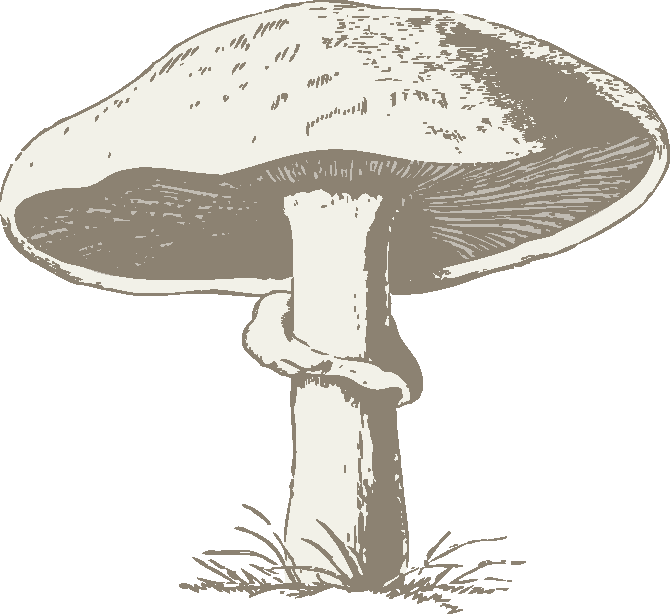
\includegraphics[width=.24\textwidth]{johnny_automatic_mushroom.pdf}
	\caption{Seta (\mushroom)}
	\label{fig:Seta}
\end{wrapfigure}
Al revisar la documentación sobre \mushroom\footnote{Ilustración obtenida en {\scriptsize\url{https://openclipart.org/detail/900/two-mushrooms-by-johnny_automatic}}} pudimos plantear mejor el problema que queríamos resolver, encontrar todas las \ARs presentes en un fichero "`pequeño"' que presenta estas características. En \urlConNotaAlPie{https://archive.ics.uci.edu/ml/datasets/Mushroom}{UCI - Machine Learning Repository} describen su origen como



\selectlanguage{english}
\begin{quote}
   Mushroom records drawn from The Audubon Society Field Guide to North American Mushrooms (1981). G. H. Lincoff (Pres.), New York: Alfred A. Knopf 
\end{quote}
\selectlanguage{spanish}
\noindent Describen brevemente el contenido del fichero, indicando que se trata de setas clasificadas como comestibles o venenosas (primer valor de cada fila).
\selectlanguage{english}
\begin{quote}
\label{cita:incertidumbre-suprimida-en-mushroom}
   This data set includes descriptions of hypothetical samples corresponding to 23 species of gilled mushrooms in the Agaricus and Lepiota Family (pp. 500-525). Each species is identified as definitely edible, definitely poisonous, or of unknown edibility and not recommended. This latter class was combined with the poisonous one. The Guide clearly states that there is no simple rule for determining the edibility of a mushroom; no rule like ``leaflets three, let it be'' for Poisonous Oak and Ivy.
\end{quote}
\selectlanguage{spanish}
\noindent Y explican los valores que puede tomar cada uno de los atributos.
\selectlanguage{english}
\begin{quote}
   \footnotesize
   1. cap-shape: bell=b, conical=c, convex=x, flat=f, knobbed=k, sunken=s
   
   2. cap-surface: fibrous=f, grooves=g, scaly=y, smooth=s

   3. cap-color: brown=n, buff=b, cinnamon=c, gray=g, green=r, pink=p, purple=u, red=e, white=w, yellow=y

   4. bruises?: bruises=t, no=f

   5. odor: almond=a, anise=l, creosote=c, fishy=y, foul=f, musty=m, none=n, pungent=p, spicy=s

   6. gill-attachment: attached=a, descending=d, free=f, notched=n

   7. gill-spacing: close=c, crowded=w, distant=d

   8. gill-size: broad=b, narrow=n

   9. gill-color: black=k, brown=n, buff=b, chocolate=h, gray=g, green=r, orange=o, pink=p, purple=u, red=e, white=w, yellow=y

   10. stalk-shape: enlarging=e, tapering=t

   11. stalk-root: bulbous=b, club=c, cup=u, equal=e, rhizomorphs=z, rooted=r, missing=?

   12. stalk-surface-above-ring: fibrous=f, scaly=y, silky=k, smooth=s

   13. stalk-surface-below-ring: fibrous=f, scaly=y, silky=k, smooth=s

   14. stalk-color-above-ring: brown=n, buff=b, cinnamon=c, gray=g, orange=o, pink=p, red=e, white=w, yellow=y

   15. stalk-color-below-ring: brown=n, buff=b, cinnamon=c, gray=g, orange=o, pink=p, red=e, white=w, yellow=y

   16. veil-type: partial=p, universal=u

   17. veil-color: brown=n, orange=o, white=w, yellow=y

   18. ring-number: none=n, one=o, two=t

   19. ring-type: cobwebby=c, evanescent=e, flaring=f, large=l, none=n, pendant=p, sheathing=s, zone=z

   20. spore-print-color: black=k, brown=n, buff=b, chocolate=h, green=r, orange=o, purple=u, white=w, yellow=y

   21. population: abundant=a, clustered=c, numerous=n, scattered=s, several=v, solitary=y

   22. habitat: grasses=g, leaves=l, meadows=m, paths=p, urban=u, waste=w, woods=d
\end{quote}
\selectlanguage{spanish}

\noindent El fichero \mushroom\footnote{\url{https://archive.ics.uci.edu/ml/machine-learning-databases/mushroom/agaricus-lepiota.data}} es un fichero de texto con 8\,124 líneas, de las que muestro aquí las tres primeras:
\begin{quote}
   \footnotesize
   p,x,s,n,t,p,f,c,n,k,e,e,s,s,w,w,p,w,o,p,k,s,u
   
   e,x,s,y,t,a,f,c,b,k,e,c,s,s,w,w,p,w,o,p,n,n,g
   
   e,b,s,w,t,l,f,c,b,n,e,c,s,s,w,w,p,w,o,p,n,n,m
\end{quote}

\noindent El fichero \mushroom con el que llevo años trabajando está codificado de otro modo, conteniendo la misma información
\begin{quote}
   \footnotesize
   1 3 9 13 23 25 34 36 38 40 52 54 59 63 67 76 85 86 90 93 98 107 113
   
   2 3 9 14 23 26 34 36 39 40 52 55 59 63 67 76 85 86 90 93 99 108 114
   
   2 4 9 15 23 27 34 36 39 41 52 55 59 63 67 76 85 86 90 93 99 108 115
\end{quote}

Este modo de registrar información sobre los individuos de una población es muy habitual en todas las ciencias. Se determina qué \atributos se pueden medir, codificándolos mediante un número reducido de valores distintos y mutuamente excluyentes, se observa a un \emph{individuo} y se mide el valor que toma en cada uno de los \atributos seleccionados, obteniendo un vector de códigos.

\begin{Definition}[Individuo]
   Sean $A_i, i = 1 \ldots n$ un conjunto de atributos, siendo $n_i$ el número de valores distintos que puede tomar el atributo $A_i$. Definimos un \emph{individuo} como una $n$-túpla, un conjunto de $n$ valores obtenidos ordenadamente de los atributos $A_i$.
   $$individuo = \left(a_1, a_2\ldots a_n\right), a_i \in A_i$$
\label{def:individuo}
\end{Definition}

El propósito de recoger esta información suele ser el de \clasificacion, clasificar al \emph{individuo} en función de los valores observados en los atributos en estudio. Esta asignación se hace en función de la información que tenemos sobre esta población, generalmente un almacén \D como \mushroom, que contiene datos sobre muchos individuos de esta población correctamente clasificados.

Aunque es un problema de \Clasificacion se trata usando \arm por la forma en que se han codificado los valores expuestos para crear el fichero \mushroom. Se han utilizado números enteros consecutivos, los dos primeros para determinar la \clase (1 = \emph{venenosa}, 2 = \emph{comestible}), los siguientes para anotar el valor del atributo \texttt{cap-shape} (3 = \emph{convex}, 4 = \emph{bell}, 5 = \emph{sunken}, 6 = \emph{flat}, 7 = \emph{knobbed}, 8 = \emph{conical}), a continuación los valores del atributo \texttt{cap-surface} (9 = \emph{smooth}, 10, 11 y 12)\ldots Si encontramos \ARs fuertes entre los atributos y la \clase podemos intentar clasificar mejor a cualquier individuo de la población.







Esta estructura permite reducir notablemente la información a procesar para extraer reglas de asociación de estos ficheros, lo que convierte su estudio en una mera ejecución con \soporte mínimo nulo (si fueran más grandes podríamos averiguar antes si no están afectados por el \dilemaIR como se ha mencionado antes). Analicemos primero la estructura y veremos después una serie de características. Para entenderlo mejor analizaremos \mushroom, que es quien nos puso sobre la pista de que algo se hacía mal con este tipo de almacenes \D.

\begin{enumerate}
	\item Tiene 8\,124 filas (a las que hemos llamado \transacciones pero llamaremos \emph{registro} a partir de ahora).
	\item Cada registro tiene 23 elementos.
   \item El primer valor de cada registro es un 1 o un 2.
         
         El segundo valor es un 3, 4, 5, 6, 7 u 8.
         
         \ldots
         
         Esto nos hace pensar que cada posición del registro representa a una variable categórica. Y descubrir que los valores utilizados para representar a una variable no coinciden con los utilizados por el resto de variables, y que estos valores son consecutivos, 1\ldots119.
   % \item Si en una fila está el 1, entonces no está el 2. Esto mismo ocurre con los grupos \{3,4,5\}, \{6,7\},\ldots \{118,119\}. Esto nos hace pensar que son los valores de diferentes \atributos o \clases. Cada fila representa el valor que un individuo toma en un determinado atributo o \clase.
\end{enumerate}

%TODO: Esto va más adelante, fuera de la INTRO
En la primera lectura de \D, la que utilizamos para crear \aprioriC[1], podemos anotar la longitud de todas las \transacciones. De este modo será muy fácil comprobar si estamos trabajando con un \catalogo.

Esto sólo lo detectamos porque se han codificado los valores de cada variable categórica de modo que no haya dos iguales y sean todos consecutivos. Basta con aplicar el algoritmo mostrado en el listado~\ref{listado:comprobarCatalogo} para averiguar si \D contiene un \catalogo, una vez leído y obtenido \aprioriC[1] y $M$, el número de valores observado en todas las \transacciones.

\lstinputlisting[label=listado:comprobarCatalogo,
                 caption={Comprobación sobre \catalogos},
                 float=htb,
                 basicstyle=\footnotesize]
                 {./contenido/clasificacion/codigo/algComprobarCatalogo}


   % \item No hay dos registros iguales. Esto nos hace pensar que se trata de un \textbf{\catalogo}, no de una \textbf{muestra}. Aunque en ambos casos la reducción de información a procesar que podemos es la misma (en la muestra\ldots) la información que obtendremos no es la misma, lo que se explica en la sección~\ref{sec:3-3-CatalogoVsMuestra}.

Un \catalogo tiene una estructura muy rígida. Si hay valores missing se puede añadir un valor al atributo en cuestión indicando esa circunstancia, o no utilizar la información del atributo en cuestión o incluso hacer una estimación del valor si se puede justificar.

En un \catalogo todos los registros contienen $n$ datos, y si forma parte de una tarea de \clasificacion uno o varios de esos datos representan una \clase, generalmente el "`\atributo"' cuyo valor queremos determinar a partir de la observación de los valores del resto de \atributos.

\begin{Definition}[Registro]
   Sean $A_i, i = 1 \ldots n$ un conjunto de atributos, siendo $n_i$ el número de valores distintos que puede tomar el atributo $A_i$. Definimos un registro como una $n$-túpla, un conjunto de $n$ valores obtenidos ordenadamente de los atributos $A_i$.
   $$registro = \left(item_1, item_2\ldots item_n\right), item_i \in A_i$$
\label{def:registro}
\end{Definition}

\begin{Definition}[\Catalogo] Un \catalogo es un conjunto de $N$ registros diferentes.
   $$\catalogo = \left\{registro_i, i = 1\ldots N\ | \ registro_i \neq registro_j \forall i \neq j\right\}$$
\label{def:catalogo}
\end{Definition}
% \borrar{Buscar una definición mejor, en \clasificacion}


El número de combinaciones entre todos los valores de los atributos en estudio es muy grande, sin embargo cuando se está haciendo un estudio real no se obtendrán todas las combinaciones posibles. En un \catalogo sólo están las combinaciones que interesa estudiar, básicamente aquellas que sí se dan en la población en estudio. Es una selección de los registros que se podrían formar con todas las combinaciones de valores proporcionada por los atributos en estudio.

La esencia de un \catalogo es que no tiene registros repetidos. Si tomamos una muestra de una población midiendo en cada individuo todos los valores de los atributos del estudio es muy probable que en la muestra existan registros repetidos. Las muestras de este tipo se verán a fondo en la sección~\ref{sec:clasificacion:catalogo:muestras}, es importante estudiar sus diferencias con los \catalogos pues contienen información sensiblemente diferente.

Un \catalogo puede cambiarse fácilmente, basta con cambiar el número de valores que puede tomar una de las variables en estudio para que cambie por completo el \catalogo. Una muestra no puede cambiarse, se obtiene de la realidad, se diseña previamente y si se quiere añadir a otra muestra en que se han utilizado otros valores debería rehacerse\ldots


Si aprovechamos esta información podemos reducir notablemente los ítems a procesar sin perder la información que contiene el \catalogo (o muestra) completo\ldots

% \borrar{Aquí viene el ejemplo de Interacción'12, he de buscar cómo escribir código.}







%\subsection{\Catalogo comprimido}
%\label{sec:3-1-1-CatalogoComprimido}
%\input{./3-ARMCatalogos/3_1_Catalogos/3_1_1_CatalogoComprimido}
%
%
%
%
%
%
%
%\subsection{Lectura de \catalogo comprimido}
%\label{sec:3-1-2-LecturaDeCatalogoComprimido}
%\input{./3-ARMCatalogos/3_1_Catalogos/3_1_2_LecturaDeCatalogoComprimido}
%
%
%










Los catálogos son colecciones de registros preparadas para resolver informáticamente un problema de clasificación. Y muchos investigadores de esta especialidad publican sus datos para que otros investigadores puedan hacer pruebas con las mismas condiciones de partida: una colección de datos con ciertas características. En UCI, KEEL, LUCS\ldots encontraremos muchos catálogos entre los datasets que publican para resolver problemas de clasificación.\marginpar{\footnotesize Acabo de descubrir LUCS, que discretiza las colecciones de UCI y me ofrece 97 valores distintos en adult, frente a los 27\,245 que tiene el de UCI, he de analizarlo con mi código y EXPLICAR MEJOR LAS CONSECUENCIAS DE APLICAR ANTES O DESPUÉS MI MÉTODO O LA AGRUPACIÓN DE VALORES EN ATRIBUTOS NUMÉRICOS ya que se obtendrán reglas y catálogos completos bastante diferentes, esto da para otro artículo y más si tengo en cuenta que tiene datos missing por lo que puedo obtener catálogos completos usando menos atributos con más registros o catálogos completos usando sólo los atributos registrados en cada registro (a no ser que el análisis nos diga que cierto atributo no aporta información\ldots.}

Cuando no sabíamos que esos ficheros contenían catálogos intentábamos aplicar bien conocidos algoritmos de ARM pero no podíamos extraer información que contienen los datos porque se desbordaba la RAM del equipo en que se está aplicando el algoritmo y se abortaba el proceso tras horas de cálculos que finalmente no obteníamos. Esto nos sorprendía porque el primer catálogo que intentamos analizar con Apriori sólo tiene 5\,644 registros de 23 datos, no son números excesivos para un problema de Minería de Datos analizado con un ordenador de escritorio con cierta potencia y capacidad de RAM. Eso nos llevó a descubrir cómo se creó el catálogo a través de \url{UCI/mushroom}\ldots

Los catálogos caracterizan un problema de clasificación concreto. Si queremos plantear otro problema de clasificación, bien etiquetando a los mismos individuos en otras \clases o bien utilizando atributos diferentes no podemos utilizar directamente cualquier catálogo que tengamos sobre la misma población. Si los dos problemas usaran los mismos atributos pero diferentes \clases y las \clases en estudio son independientes no servirá de nada la información que tengamos sobre los catálogos completos del primer problema de clasificación si no sabemos analizar qué información puede ser relevante y cuál no, de hecho la información menos relevante en esta situación es la distribución de las \clases en cada uno de los problemas de clasificación por lo que debemos huir de interpretaciones erróneas utilizando estos datos para estimar soportes o confianzas poblacionales.

De un catálogo se puede extraer información válida para otro problema de clasificación que utilice los mismos atributos ya que si en la muestra en que se basa el catálogo no presenta cierta relación entre los valores de los atributos YA SABEMOS QUE NO APARECERÁ ESA RELACIÓN AUNQUE CAMBIEMOS DE CLASES (siempre que el catálogo sea válido, aún tengo que hacer muchas definiciones sobre muestra, población, distribución de \clases, problema de \clasificacion, \atributos, \clases, \catalogos, catálogos completos, validez de un catálogo\ldots).

Aunque la \ARM busca cualquier relación entre cualquier par (o $k$-itemset) de valores de \D, el objetivo del problema de \clasificacion es siempre el mismo, etiquetar cada \registro con una \clase basándose en la información disponible sobre otros \registros con valores idénticos en sus \atributos.





\subsection{Muestras}
\label{sec:clasificacion:catalogo:muestras}
La importancia que se da en todos los estudios de \ARM al \soporte de una \ar se justifica cuando se trabaja con muestras, que no contienen la misma información que un \catalogo. Para obtener una muestra en un problema de \clasificacion se han de seleccionar individuos de una población, medir en cada uno de ellos el valor que toma cada uno de los \atributos en estudio y averiguar la \clase a la que pertenece. Al guardar todos los \registros obtenidos de este modo es posible que existan \registros repetidos, lo que aporta información sobre la distribución de la población en estudio con un elevado coste sobre los \catalogos ya que en estos no deberíamos repetir el registro si no añadir un número entero indicando el número de veces que aparece el \registro en la muestra.

